% !TeX spellcheck = ru_RU
% !TEX root = vkr.tex

\section{Описание решения}

В данном разделе рассмотрены различные подходы к решению задачи мониторинга,
описаны алгоритм обработки видеозаписей и процесс создания единого сервиса с \texttt{Telegram}-ботом для рассылки,
а также представлена инструкция по обучению модели на данных конкретного объекта.

% Реализация в широком смысле: что таки было сделано.
% Часто это на самом деле несколько отдельных разделов, по одному на каждую \enquote{реализационную} задачу из постановки.
% Например, \enquote{Архитектура} и \enquote{Особенности реализации}, либо по разделу на каждую крупную подзадачу.
% Если разделы получились недостаточно эпичными (меньше пары страниц), сделайте их подразделами одного большого раздела, как тут.

% Если программной реализации нет, тут пишутся Ваши теоретические наработки, если есть, хоть в каком-то виде, то опишите, даже если серьёзно кодом надо будет заняться только в следующей части.

% Если работа на текущем этапе предполагает \emph{только} обзор, то
% \begin{itemize}
%     \item но всё равно же надо было попробовать воспроизвести чужие результаты, напишите про это сюда;
%     \item если нет, то, наверное, обзор получился годным и ценным сам по себе, источников 40--50 было рассмотрено%
%           \footnote{Это не шутка, в хороших работах, где целый семестр делался только обзор, оно примерно так и выходит.},
%           тогда ладно, раздел \enquote{Описание решения} можно не делать.
% \end{itemize}

% Для понимания того, как отчёт по учебной практике должен писаться, можно посмотреть видео ниже.
% Они про научные доклады и написание научных статей.
% Учебные практики и ВКР отличаются тем, что тут есть требования отдельных глав (слайдов) со списком задач и списком результатов.
% Но даже если Вы забьёте на требования, специфичные для ВКР, и соблюдете все рекомендации ниже, получившиеся скорее всего будет лучше, чем первая попытка 99\% ваших однокурсников.

% \begin{enumerate}
%     \item \enquote{Как сделать великолепный научный доклад} от Саймона Пейтона Джонса~\cite{SPJGreatTalk} (на английском).
%     \item \enquote{Как написать великолепную научную статью} от Саймона Пейтона Джонса~\cite{SPJGreatPaper} (на английском).
%     \item \enquote{Как писать статьи так, чтобы люди их смогли прочитать} от Дэрэка Драйера~\cite{DreyerYoutube2020} (на английском).
%           По предыдущим ссылкам разбирается, что должно быть в статье, т.е. как она должна выгля\-деть на высоком уровне.
%           Тут более низкоуровнево изложено, как должны быть устроены параграфы и т.п.
%     \item Или на русском от С.~Григорьева~\cite{SemenI,SemenII}.
%     \item Ещё можно посмотреть How to Design Talks~\cite{JhalaYoutube2020} от Ranjit Jhala, но мы думаем, что первых ссылок всем хватит.
% \end{enumerate}

% Можно глянуть примеры хороших работ прошлых лет на сайте кафедры системного программирования%
% \footnote{Сайт кафедры СП, архив практик и ВКР: URL: \url{https://se.math.spbu.ru/theses.html} (дата обращения: \DTMdate{2024-01-15}).}.
% Например, работа Москаленко Ивана Николаевича за 3-й курс%
% \footnote{\enquote{Создание базы данных изображений для глобальной локализации в пространстве}, URL: \url{https://se.math.spbu.ru/thesis_download?thesis_id=1199} (дата обращения: \DTMdate{2024-01-15}).}.

\subsection{Способы получения статистик}
\label{subsec:getting_data_from_objects}

В данной работе система была рассчитана на использование одной камеры на объекте,
поэтому возникали ограничения, накладываемые на проект.
К примеру, нельзя просто подсчитывать количество всех людей и машин в кадре,
находившихся в зоне строительного объекта,
так как на объекте могли быть слепые зоны или они могли появиться в процессе строительства.
Также, поскольку система была рассчитана на экономное подключение, могли использоваться стандартные камеры с плохим разрешением,
что ухудшало предсказания детекции.

Было решено отслеживать определённую зону, которую рабочие и техника проходили как при входе, так и при выходе.
Чаще всего это зона ворот или аналогичная часть объекта. Данный подход имел несколько преимуществ:

\begin{enumerate}
      \item Зона ворот на камере всегда должна просматриваться,
      так как иначе служба охраны не сможет качественно выполнять свою работу.
      Из этого следует, что слепые зоны не мешали при таком подходе.
      Поэтому просматриваемость ворот для данной работы считается требованием.
      \item Даже при низком качестве камеры после дообучения модели
      и при грамотной настройке трекера системе было достаточно один раз обнаружить объект,
      а трекер мог самостоятельно предсказывать положение объекта, что повышало устойчивость.
\end{enumerate}

У данного подхода также был серьёзный недостаток: если ворот на объекте несколько
или существуют иные способы уйти с объекта или зайти на него, данный подход не сможет корректно посчитать статистику.
Решением этой проблемы может стать подключение второй камеры или подача второй зоны ворот из первого видео,
но тогда решение будет требовать небольших доработок.

\subsection{Создание ML pipeline для обработки видео}
\label{subsec:creating_ml_pipeline}

Далее описано, как работал \texttt{ML pipeline} в данной работе.
Он был представлен отдельным сервисом, который принимал заявки на обработку видео
и возвращал файл для подготовки статистического отчёта.

% ML-пайплайн обработки одной видеозаписи смены.
% Подключение в текст: % ML-пайплайн обработки одной видеозаписи смены.
% Подключение в текст: % ML-пайплайн обработки одной видеозаписи смены.
% Подключение в текст: \input{figures/ml_pipeline}
\begin{figure}[H]
    \centering
    \begin{tikzpicture}[
        font=\small,
        node distance=18mm and 7mm,
        stage/.style={draw, rounded corners=2pt, minimum height=14mm, text width=28mm, align=center, inner sep=3pt, fill=blue!7},
        model/.style={stage, fill=orange!15},
        result/.style={stage, fill=green!10},
        config/.style={draw, dashed, rounded corners=2pt, text width=34mm, align=center, inner sep=3pt, fill=gray!8},
        flow/.style={->, >=latex, thick},
        control/.style={->, >=latex, dashed, gray!75, thick}
    ]
        \node[stage] (video) {Видеозапись смены};
        \node[stage, right=of video] (roi) {Обрезка по ROI};
        \node[model, right=of roi] (detect) {Детекция объектов};
        \node[model, right=of detect] (track) {Работа трекера};

        \node[stage, below=of track] (line) {Контроль пересечения линии};
        \node[result, left=of line] (event) {Запись о пересечении};
        \node[result, left=of event] (report) {Создание отчёта};

        \node[config, above=of detect] (project) {Конфигурация объекта};

        \draw[flow] (video) -- (roi);
        \draw[flow] (roi) -- (detect);
        \draw[flow] (detect) -- (track);
        \draw[flow] (track) -- (line);
        \draw[flow] (line) -- (event);
        \draw[flow] (event) -- (report);

        \draw[control] (project.south west) -- (roi.north);
        \draw[control] (project.south) -- (detect.north);
        \draw[control] (project.south east) -- (track.north);
        \draw[control] (project.east) -| ([xshift=8mm]line.east) -- (line.east);
    \end{tikzpicture}
    \caption{ML-пайплайн обработки видеозаписи строительного объекта.}
    \label{fig:ml-pipeline}
\end{figure}

\begin{figure}[H]
    \centering
    \begin{tikzpicture}[
        font=\small,
        node distance=18mm and 7mm,
        stage/.style={draw, rounded corners=2pt, minimum height=14mm, text width=28mm, align=center, inner sep=3pt, fill=blue!7},
        model/.style={stage, fill=orange!15},
        result/.style={stage, fill=green!10},
        config/.style={draw, dashed, rounded corners=2pt, text width=34mm, align=center, inner sep=3pt, fill=gray!8},
        flow/.style={->, >=latex, thick},
        control/.style={->, >=latex, dashed, gray!75, thick}
    ]
        \node[stage] (video) {Видеозапись смены};
        \node[stage, right=of video] (roi) {Обрезка по ROI};
        \node[model, right=of roi] (detect) {Детекция объектов};
        \node[model, right=of detect] (track) {Работа трекера};

        \node[stage, below=of track] (line) {Контроль пересечения линии};
        \node[result, left=of line] (event) {Запись о пересечении};
        \node[result, left=of event] (report) {Создание отчёта};

        \node[config, above=of detect] (project) {Конфигурация объекта};

        \draw[flow] (video) -- (roi);
        \draw[flow] (roi) -- (detect);
        \draw[flow] (detect) -- (track);
        \draw[flow] (track) -- (line);
        \draw[flow] (line) -- (event);
        \draw[flow] (event) -- (report);

        \draw[control] (project.south west) -- (roi.north);
        \draw[control] (project.south) -- (detect.north);
        \draw[control] (project.south east) -- (track.north);
        \draw[control] (project.east) -| ([xshift=8mm]line.east) -- (line.east);
    \end{tikzpicture}
    \caption{ML-пайплайн обработки видеозаписи строительного объекта.}
    \label{fig:ml-pipeline}
\end{figure}

\begin{figure}[H]
    \centering
    \begin{tikzpicture}[
        font=\small,
        node distance=18mm and 7mm,
        stage/.style={draw, rounded corners=2pt, minimum height=14mm, text width=28mm, align=center, inner sep=3pt, fill=blue!7},
        model/.style={stage, fill=orange!15},
        result/.style={stage, fill=green!10},
        config/.style={draw, dashed, rounded corners=2pt, text width=34mm, align=center, inner sep=3pt, fill=gray!8},
        flow/.style={->, >=latex, thick},
        control/.style={->, >=latex, dashed, gray!75, thick}
    ]
        \node[stage] (video) {Видеозапись смены};
        \node[stage, right=of video] (roi) {Обрезка по ROI};
        \node[model, right=of roi] (detect) {Детекция объектов};
        \node[model, right=of detect] (track) {Работа трекера};

        \node[stage, below=of track] (line) {Контроль пересечения линии};
        \node[result, left=of line] (event) {Запись о пересечении};
        \node[result, left=of event] (report) {Создание отчёта};

        \node[config, above=of detect] (project) {Конфигурация объекта};

        \draw[flow] (video) -- (roi);
        \draw[flow] (roi) -- (detect);
        \draw[flow] (detect) -- (track);
        \draw[flow] (track) -- (line);
        \draw[flow] (line) -- (event);
        \draw[flow] (event) -- (report);

        \draw[control] (project.south west) -- (roi.north);
        \draw[control] (project.south) -- (detect.north);
        \draw[control] (project.south east) -- (track.north);
        \draw[control] (project.east) -| ([xshift=8mm]line.east) -- (line.east);
    \end{tikzpicture}
    \caption{ML-пайплайн обработки видеозаписи строительного объекта.}
    \label{fig:ml-pipeline}
\end{figure}


Для хранения конфигурации объектов использовалась \texttt{PostgreSQL}~\footnote{Документация \texttt{PostgreSQL}: \url{https://www.postgresql.org/docs/} (дата обращения: \DTMdate{2026-09-25}).}, которая являлась удобной СУБД и также использовалась далее в работе.

Для повышения качества модель была обучена на обрезанных изображениях с зоной ворот,
так как объекты были крупнее, чем на исходном изображении.
В качестве модели детекции была выбрана именно модель семейства \texttt{YOLO}.
Она обеспечила обработку видео в режиме \texttt{real-time}, имела хорошее качество детекции и удобный интерфейс обучения и инференса.
В качестве аналога можно взять \texttt{RT-DETR}. \texttt{RT-DETR} из-за своей архитектуры более требовательна
и имеет меньшую скорость работы по сравнению с \texttt{YOLO},
но может показать более высокие метрики в некоторых случаях.

Далее модель передавала результаты детекции трекеру. Решено было взять \texttt{ByteTrack},
так как его можно использовать через библиотеку \texttt{Supervision}~\footnote{Документация библиотеки \texttt{Supervision}: \url{https://supervision.roboflow.com/} (дата обращения: \DTMdate{2026-09-25}).},
на которой была реализована большая часть \texttt{ML pipeline}.
Также он значительно проще в настройке по сравнению с другими трекерами из этой же библиотеки.
Для более качественного результата рекомендуется использовать \texttt{BoT-SORT}:
его также можно использовать через \texttt{Supervision}, но главное преимущество --- он содержит эмбеддинг-модель,
что делает его более точным и устойчивым, но сложным к настройке.

Вход и выход работников и техники на объект отслеживались через пересечение заданной линии.
Такой функционал есть в библиотеке \texttt{Supervision}.
При пересечении линии объектом в статистику добавлялась соответствующая запись.

Итоговый подсчёт статистики выполнялся отдельно после обработки всей смены: рассчитывались показатели и формировались графики.
Недостаток данного метода заключается в том, что в течение дня одни и те же сотрудники могли выходить и заходить на объект,
но при учёте этого в подсчёте статистики проблема не возникала.

\subsection{Создание backend-сервиса}
\label{subsec:creating_system_arch}

Архитектура проекта разделена на два сервиса: один из них --- описанный выше \texttt{ML}-сервис, а другой ---
\texttt{backend}-сервис. В этом разделе будет подробно описана именно часть, связанная с \texttt{backend}.

% Взаимодействие backend- и ML-сервисов.
% Подключение в текст: % Взаимодействие backend- и ML-сервисов.
% Подключение в текст: % Взаимодействие backend- и ML-сервисов.
% Подключение в текст: \input{figures/system_pipeline}
\begin{figure}[H]
    \centering
    \begin{tikzpicture}[
        scale=0.80, transform shape, font=\small,
        component/.style={draw, rounded corners=2pt, minimum height=10mm, text width=27mm, align=center, inner sep=3pt, fill=white},
        camera/.style={component, fill=gray!10, text width=20mm},
        storage/.style={component, fill=green!10, text width=24mm},
        backend/.style={draw=blue!65, rounded corners=3pt, thick, fill=blue!4},
        ml/.style={draw=orange!80!black, rounded corners=3pt, thick, fill=orange!8},
        flow/.style={->, >=latex, thick}
    ]
        % Backend-сервис.
        \draw[backend] (-4.3,2.4) rectangle (0.3,-3.0);
        \node[font=\bfseries] at (-2.0,2.0) {Backend-сервис};
        \node[component] (recorder) at (-2.0,0.7) {Планировщик и запись видео};
        \node[component] (reports) at (-2.0,-1.5) {API и сервис отчётов};

        % ML-сервис.
        \draw[ml] (4.5,2.4) rectangle (8.5,-3.0);
        \node[font=\bfseries] at (6.5,2.0) {ML-сервис};
        \node[component] (processor) at (6.5,-0.4) {Обработка видео};

        % Несколько источников видеопотока.
        \node[camera] (camera1) at (-7.0,1.8) {Камера 1};
        \node[camera] (camera2) at (-7.0,0.7) {Камера 2};
        \node[font=\Large] at (-7.0,-0.25) {$\vdots$};
        \node[camera] (cameran) at (-7.0,-1.2) {Камера N};

        % Очередь между сервисами, база данных и получатель отчёта.
        \node[storage] (queue) at (2.25,0.7) {Redis / RQ};
        \node[storage] (database) at (2.25,-1.5) {PostgreSQL};
        \node[camera] (telegram) at (-7.0,-3.3) {Telegram};

        % Сбор видео и постановка задачи на обработку.
        \draw[flow] (camera1.east) -- (recorder.west);
        \draw[flow] (camera2.east) -- (recorder.west);
        \draw[flow] (cameran.east) -- (recorder.west);
        \draw[flow] (recorder.east) -- (queue.west);
        \draw[flow] (recorder.east) -- (database.west);

        % Обработка и возврат результата.
        \draw[flow] (queue.east) -- (processor.west);
        \draw[flow] (processor.west) -- (database.east);

        % Получение результата и отправка отчёта.
        \draw[flow] (database.west) -- (reports.east);
        \draw[flow] (reports.west) -- (telegram.east);
    \end{tikzpicture}
    \caption{Взаимодействие backend- и ML-сервисов при параллельной записи видеопотоков с камер строительного объекта.}
    \label{fig:system-pipeline}
\end{figure}

\begin{figure}[H]
    \centering
    \begin{tikzpicture}[
        scale=0.80, transform shape, font=\small,
        component/.style={draw, rounded corners=2pt, minimum height=10mm, text width=27mm, align=center, inner sep=3pt, fill=white},
        camera/.style={component, fill=gray!10, text width=20mm},
        storage/.style={component, fill=green!10, text width=24mm},
        backend/.style={draw=blue!65, rounded corners=3pt, thick, fill=blue!4},
        ml/.style={draw=orange!80!black, rounded corners=3pt, thick, fill=orange!8},
        flow/.style={->, >=latex, thick}
    ]
        % Backend-сервис.
        \draw[backend] (-4.3,2.4) rectangle (0.3,-3.0);
        \node[font=\bfseries] at (-2.0,2.0) {Backend-сервис};
        \node[component] (recorder) at (-2.0,0.7) {Планировщик и запись видео};
        \node[component] (reports) at (-2.0,-1.5) {API и сервис отчётов};

        % ML-сервис.
        \draw[ml] (4.5,2.4) rectangle (8.5,-3.0);
        \node[font=\bfseries] at (6.5,2.0) {ML-сервис};
        \node[component] (processor) at (6.5,-0.4) {Обработка видео};

        % Несколько источников видеопотока.
        \node[camera] (camera1) at (-7.0,1.8) {Камера 1};
        \node[camera] (camera2) at (-7.0,0.7) {Камера 2};
        \node[font=\Large] at (-7.0,-0.25) {$\vdots$};
        \node[camera] (cameran) at (-7.0,-1.2) {Камера N};

        % Очередь между сервисами, база данных и получатель отчёта.
        \node[storage] (queue) at (2.25,0.7) {Redis / RQ};
        \node[storage] (database) at (2.25,-1.5) {PostgreSQL};
        \node[camera] (telegram) at (-7.0,-3.3) {Telegram};

        % Сбор видео и постановка задачи на обработку.
        \draw[flow] (camera1.east) -- (recorder.west);
        \draw[flow] (camera2.east) -- (recorder.west);
        \draw[flow] (cameran.east) -- (recorder.west);
        \draw[flow] (recorder.east) -- (queue.west);
        \draw[flow] (recorder.east) -- (database.west);

        % Обработка и возврат результата.
        \draw[flow] (queue.east) -- (processor.west);
        \draw[flow] (processor.west) -- (database.east);

        % Получение результата и отправка отчёта.
        \draw[flow] (database.west) -- (reports.east);
        \draw[flow] (reports.west) -- (telegram.east);
    \end{tikzpicture}
    \caption{Взаимодействие backend- и ML-сервисов при параллельной записи видеопотоков с камер строительного объекта.}
    \label{fig:system-pipeline}
\end{figure}

\begin{figure}[H]
    \centering
    \begin{tikzpicture}[
        scale=0.80, transform shape, font=\small,
        component/.style={draw, rounded corners=2pt, minimum height=10mm, text width=27mm, align=center, inner sep=3pt, fill=white},
        camera/.style={component, fill=gray!10, text width=20mm},
        storage/.style={component, fill=green!10, text width=24mm},
        backend/.style={draw=blue!65, rounded corners=3pt, thick, fill=blue!4},
        ml/.style={draw=orange!80!black, rounded corners=3pt, thick, fill=orange!8},
        flow/.style={->, >=latex, thick}
    ]
        % Backend-сервис.
        \draw[backend] (-4.3,2.4) rectangle (0.3,-3.0);
        \node[font=\bfseries] at (-2.0,2.0) {Backend-сервис};
        \node[component] (recorder) at (-2.0,0.7) {Планировщик и запись видео};
        \node[component] (reports) at (-2.0,-1.5) {API и сервис отчётов};

        % ML-сервис.
        \draw[ml] (4.5,2.4) rectangle (8.5,-3.0);
        \node[font=\bfseries] at (6.5,2.0) {ML-сервис};
        \node[component] (processor) at (6.5,-0.4) {Обработка видео};

        % Несколько источников видеопотока.
        \node[camera] (camera1) at (-7.0,1.8) {Камера 1};
        \node[camera] (camera2) at (-7.0,0.7) {Камера 2};
        \node[font=\Large] at (-7.0,-0.25) {$\vdots$};
        \node[camera] (cameran) at (-7.0,-1.2) {Камера N};

        % Очередь между сервисами, база данных и получатель отчёта.
        \node[storage] (queue) at (2.25,0.7) {Redis / RQ};
        \node[storage] (database) at (2.25,-1.5) {PostgreSQL};
        \node[camera] (telegram) at (-7.0,-3.3) {Telegram};

        % Сбор видео и постановка задачи на обработку.
        \draw[flow] (camera1.east) -- (recorder.west);
        \draw[flow] (camera2.east) -- (recorder.west);
        \draw[flow] (cameran.east) -- (recorder.west);
        \draw[flow] (recorder.east) -- (queue.west);
        \draw[flow] (recorder.east) -- (database.west);

        % Обработка и возврат результата.
        \draw[flow] (queue.east) -- (processor.west);
        \draw[flow] (processor.west) -- (database.east);

        % Получение результата и отправка отчёта.
        \draw[flow] (database.west) -- (reports.east);
        \draw[flow] (reports.west) -- (telegram.east);
    \end{tikzpicture}
    \caption{Взаимодействие backend- и ML-сервисов при параллельной записи видеопотоков с камер строительного объекта.}
    \label{fig:system-pipeline}
\end{figure}


Для сбора данных \texttt{backend}-сервис по расписанию подключался к \texttt{RTSP}-стримам и
сохранял видеозаписи в хранилище. Для фиксации дальнейших действий в базе данных \texttt{PostgreSQL}
создавалась запись с идентификатором объекта, временем начала и окончания смены,
статусом записи и путём к сохранённому видео.

После завершения записи \texttt{backend} создавал задачу обработки
и помещал её в очередь \texttt{Redis}~\footnote{Документация \texttt{Redis}: \url{https://redis.io/docs/latest/} (дата обращения: \DTMdate{2026-09-25}).} с использованием \texttt{RQ}~\footnote{Документация \texttt{RQ}: \url{https://python-rq.org/docs/} (дата обращения: \DTMdate{2026-09-25}).}. Такой подход позволил
записывать несколько видеозаписей одновременно и обрабатывать их все одним \texttt{ML}-сервисом.
Также эту реализацию можно улучшить, например, добавив ещё \texttt{ML}-сервисы,
которые будут брать задачи на обработку, или при наличии разных моделей добавить параметр,
который позволит ожидать определённый \texttt{ML}-сервис.

\texttt{ML}-сервис описан выше: он брал задачу из очереди,
подгружал параметры и выполнял обработку, после чего заносил в \texttt{PostgreSQL} информацию о результате.

После успешной обработки всех смен за день \texttt{backend}-сервис получал результаты из
\texttt{PostgreSQL}, объединял их в итоговую таблицу и формировал отчёт. Подготовленный
файл вместе с текстовой сводкой и графиками отправлялся подписанным получателям
через \texttt{Telegram}-бота~\footnote{Документация \texttt{Telegram Bot API}: \url{https://core.telegram.org/bots/api} (дата обращения: \DTMdate{2026-09-25}).}.

\texttt{Telegram}-бот реализован для отправки сообщений пользователям, которые хотя бы раз написали ему.
Этот базовый функционал позволяет расширить бота и адаптировать его к дополнительным требованиям.

\subsection{Создание статистического отчёта}
\label{subsec:creating_report}

Статистический отчёт должен быть небольшим, информативным и не вводящим в заблуждение.
Выше уже была описана проблема: в предложенном подходе работники и техника,
которые выходят и заходят на объект, могли дополнительно увеличивать счётчик количества заходов и выходов,
поэтому использовать эти величины в качестве статистики --- плохая идея.

Для данного проекта одним из наиболее информативных показателей являлось среднее количество работников и техники в течение рабочего дня. Также стоит отметить,
что рассчитывать статистику за полный рабочий день не имеет большого смысла: ночью количество персонала будет значительно ниже, чем днём,
поэтому логичнее разбивать видео со смены на несколько частей, соответствующих времени работы смен работников.

\[
    \overline{N} = \frac{1}{T_{\text{см}}}\int_{\tau_0}^{\tau_{m+1}} N(t)\,dt
    \approx \frac{1}{T_{\text{см}}}\sum_{i=0}^{m} N_i\bigl(\tau_{i+1}-\tau_i\bigr),
    \qquad T_{\text{см}} = \tau_{m+1}-\tau_0.
\]
где
\begin{itemize}
    \item $\overline{N}$ --- среднее количество людей за смену;
    \item $T_{\text{см}}$ --- длительность смены;
    \item $N(t)$ --- количество людей на объекте в момент времени $t$;
    \item $\tau_0$ и $\tau_{m+1}$ --- время начала и окончания смены соответственно;
    \item $\tau_i$ --- время $i$-й записи о пересечении линии;
    \item $N_i$ --- количество людей в начале интервала $[\tau_i, \tau_{i+1})$;
    \item $m$ --- количество записей о пересечении линии за смену.
\end{itemize}

Дополнительно к среднему значению в этом проекте был построен график зависимости среднего значения за определённый час от времени. Это позволило при желании уточнить,
когда прибывала техника и когда рабочие находились на объекте.

\begin{figure}[H]
    \centering
    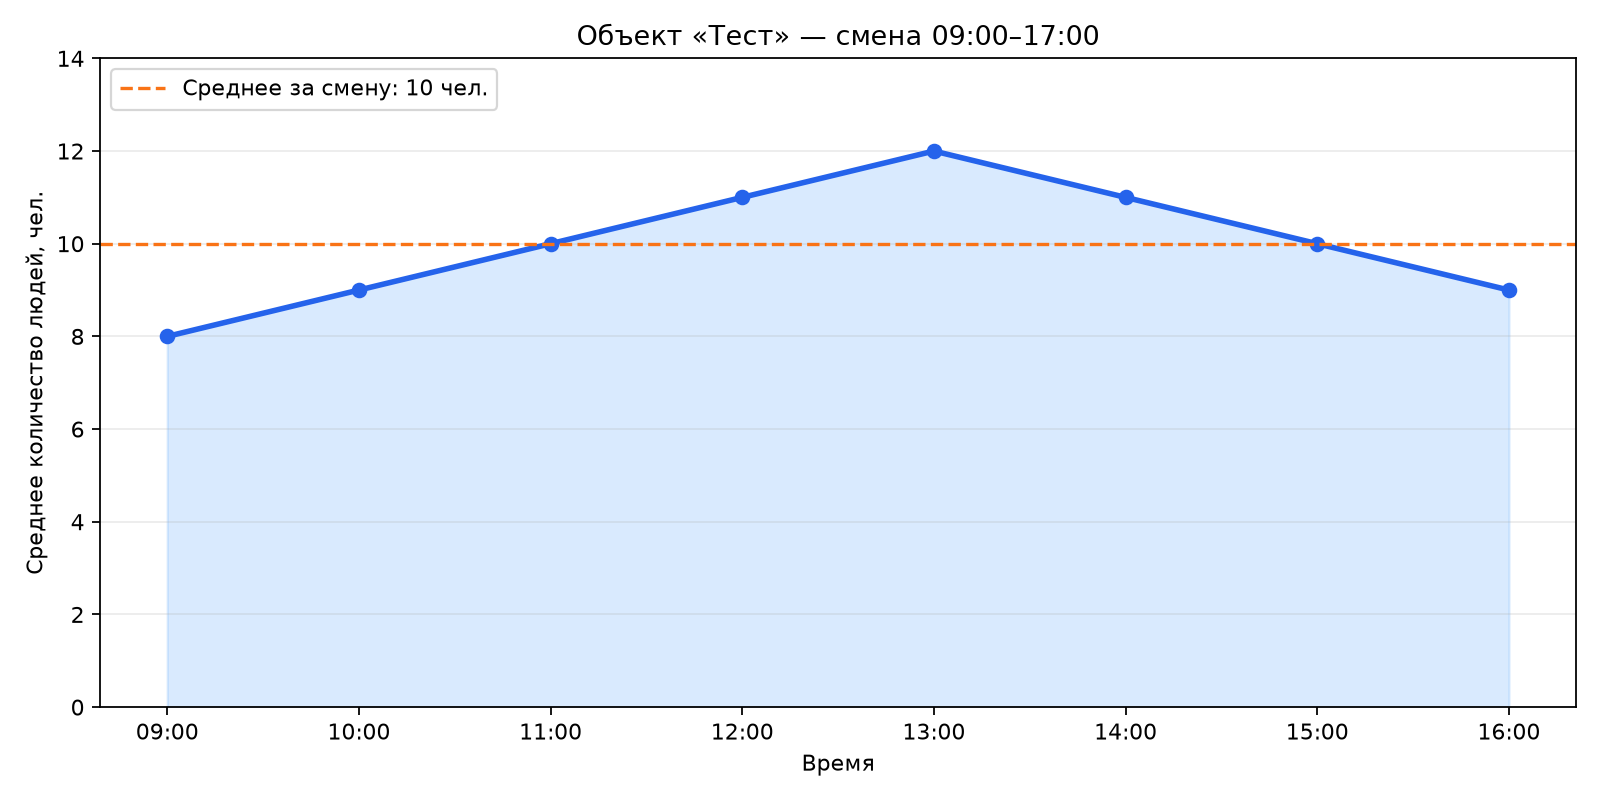
\includegraphics[width=0.88\textwidth]{../assets/test_personnel_example.png}
    \caption{Пример графика статистического отчёта за смену}
    \label{fig:shift-report-chart-example}
\end{figure}

\subsection{Описание экспериментов}

В этой работе были проведены эксперименты по обучению модели под домен строительных объектов,
а также эксперимент по замеру end-to-end качества сервиса.

Для тонкой настройки модели \texttt{YOLO} использовался датасет \texttt{MOCS}~\footnote{Датасет \texttt{MOCS}: \url{https://www.kaggle.com/datasets/xiaopan9802/mocs-dataset} (дата обращения: \DTMdate{2026-09-28}).}.
Он содержит разные виды техники и рабочих, что соответствует доменной области.

Для измерения end-to-end-качества использовался датасет \texttt{CMOT}~\footnote{Датасет \texttt{CMOT}: \url{https://github.com/XZ-YAN/CMOT-Dataset} (дата обращения: \DTMdate{2026-09-28}).}.
Он содержит записи со строительных объектов, где отмечены траектории рабочих и строительной техники.

% \subsection{Создание инструкции для обучение модели}

% Для нового проекта лучше будет адаптировать предобученную модель под конкретную задачу.
% Интерфейс \texttt{ultralytics} очень удобен для быстрого обучения,
% для этого нужно создать yaml файл по шаблону и передать его модели.

% Для обучения нужно выбрать гиперпараметры,

% \subsection{Некоторые типичные ошибки}
% Здесь мы будем собирать основные ошибки, которые случаются при написании текстов.
% В интернетах тоже можно найти коллекции типич\-ных косяков%
% \footnote{\href{https://www.read.seas.harvard.edu/~kohler/latex.html}{https://www.read.seas.harvard.edu/\textasciitilde kohler/latex.html} (дата обращения: \DTMdate{2022-12-16}).}.

% Рекомендуется по-умоЗдесь мы будем собирать основные ошибки, которые случаются при написании текстов.
% В интернетах тоже можно найти коллекции типич\-ных косяков%
% \footnote{\href{https://www.read.seas.harvard.edu/~kohler/latex.html}{https://www.read.seas.harvard.edu/\textasciitilde kohler/latex.html} (дата обращения: \DTMdate{2022-12-16}).}.

% Рекомендуется по-умол\-ча\-нию использовать красивые греческие бук\-вы $\sigma$  и $\phi$, а именно $\phi$ вместо $\varphi$.
% В данном шаблоне команды для этих букв переставлены местами по сравнению с ванильным \TeX'ом.

% Также, если работа пишется на русском языке, необходимо, чтобы работа была написана на \textit{грамотном} русском языке даже если автор из ближнего зарубежья%
% \footnote{Теоретически, возможен вариант написания текстов на английском языке, но это необходимо обсудить в первую очередь с научным руководителем.}.
% Это включает в себя:
% \begin{itemize}
%     \item разделы должны оформляться с помощью \verb=\section{...}=, а также \verb=\subsection= и т.~п.; не нужно пытаться нумеровать вручную;
%     \item точки после окончания предложений должны присутствовать;
%     \item пробелы после запятых и точек, в конце слова перед скобкой;
%     \item неразрывные пробелы там, где нужны пробелы, но переносить на другую строку нельзя, например \verb=т.~е.=, \verb=А.~Н.~Терехов=, \verb=что-то~\cite{?}=, \verb=что-то~\ref{?}=;
%     \item дефис там, где нужен дефис (обозначается с помощью одиночного \enquote{минуса} (англ. dash) на клавиатуре);
%     \item двойной дефис там, где он нужен; а именно  при указании проме\-жутка в цифрах: в 1900--1910 г.~г., стр. 150--154;
%     \item тире (т.~е. \verb=---=~--- тройной минус) на месте тире, а не что-то другое; в русском языке тире не может \enquote{съезжать} на новую строку, поэтому стоит использовать такой синтаксис: \verb=До~--- после=;
%     \item даты стоит писать везде одинаково; чтобы об этом не следить, можно пользоваться заклинанием \verb=\DTMdate{2022-12-16}=;
%     \item правильные кавычки должны набираться с помощью пакета \texttt{csquotes}: для основного языка в \texttt{polyglossia} стоит использовать команду \verb=\enquote{текст}=, для второго языка стоит использовать \verb=\foreignquote{язык}{текст}=; правильные кавычки в русской типографии~--- \verb=<<ёлочки>>=, ни в коем случае не \verb="скандинавские лапки"=;
%     \item все перечисления должны оформляться с помощью \verb=\enumerate= или \verb=\itemize=; пункты перечислений должны либо начинаться с заглавной буквы и заканчиваться точкой, либо начинаться со строчной и закачиваться точкой с запятой; последний пункт пере\-числений всегда заканчивается точкой.
%     \item Перед выкладыванием финальной версии необходимо просмотреть лог \LaTeX'a, и обратить внимание на сообщения вида \emph{Overfull \textbackslash hbox (1.29312pt too wide) in paragraph}. Обычно, это означает, что текст выползает за поля, и надо подсказать, как правильно разделять слова на слоги, чтобы перенос произошел автоматически.
%           Это делается, например, так: \verb=соломо\-волокуша=.
%     \item \emph{Обязательно используйте инструменты автоматической проверки правописания!}
%           Не посылайте текст даже научному руководителю на проверку, если не прогнали спеллчекер%
%           \footnote{Например, для браузера можно использовать плагин LanguageTool, для VS Code --- Code Spell Checker с расширением для русского (но он вроде не умеет пунктуацию, так что следите за запятыми).}%
%           , желательно, умеющий проверять пунктуацию~--- у научника куча времени уйдёт на комментарии вида \enquote{тут нужна запятая} и не останется сил посоветовать что-нибудь по делу.
%           А ещё научник будет шокирован уровнем грамотности современной молодёжи, впадёт в депрессию и не будет отвечать вам неделю.
% \end{itemize}
% л\-ча\-нию использовать красивые греческие бук\-вы $\sigma$  и $\phi$, а именно $\phi$ вместо $\varphi$.
% В данном шаблоне команды для этих букв переставлены местами по сравнению с ванильным \TeX'ом.

% Также, если работа пишется на русском языке, необходимо, чтобы работа была написана на \textit{грамотном} русском языке даже если автор из ближнего зарубежья%
% \footnote{Теоретически, возможен вариант написания текстов на английском языке, но это необходимо обсудить в первую очередь с научным руководителем.}.
% Это включает в себя:
% \begin{itemize}
%     \item разделы должны оформляться с помощью \verb=\section{...}=, а также \verb=\subsection= и т.~п.; не нужно пытаться нумеровать вручную;
%     \item точки после окончания предложений должны присутствовать;
%     \item пробелы после запятых и точек, в конце слова перед скобкой;
%     \item неразрывные пробелы там, где нужны пробелы, но переносить на другую строку нельзя, например \verb=т.~е.=, \verb=А.~Н.~Терехов=, \verb=что-то~\cite{?}=, \verb=что-то~\ref{?}=;
%     \item дефис там, где нужен дефис (обозначается с помощью одиночного \enquote{минуса} (англ. dash) на клавиатуре);
%     \item двойной дефис там, где он нужен; а именно  при указании проме\-жутка в цифрах: в 1900--1910 г.~г., стр. 150--154;
%     \item тире (т.~е. \verb=---=~--- тройной минус) на месте тире, а не что-то другое; в русском языке тире не может \enquote{съезжать} на новую строку, поэтому стоит использовать такой синтаксис: \verb=До~--- после=;
%     \item даты стоит писать везде одинаково; чтобы об этом не следить, можно пользоваться заклинанием \verb=\DTMdate{2022-12-16}=;
%     \item правильные кавычки должны набираться с помощью пакета \texttt{csquotes}: для основного языка в \texttt{polyglossia} стоит использовать команду \verb=\enquote{текст}=, для второго языка стоит использовать \verb=\foreignquote{язык}{текст}=; правильные кавычки в русской типографии~--- \verb=<<ёлочки>>=, ни в коем случае не \verb="скандинавские лапки"=;
%     \item все перечисления должны оформляться с помощью \verb=\enumerate= или \verb=\itemize=; пункты перечислений должны либо начинаться с заглавной буквы и заканчиваться точкой, либо начинаться со строчной и закачиваться точкой с запятой; последний пункт пере\-числений всегда заканчивается точкой.
%     \item Перед выкладыванием финальной версии необходимо просмотреть лог \LaTeX'a, и обратить внимание на сообщения вида \emph{Overfull \textbackslash hbox (1.29312pt too wide) in paragraph}. Обычно, это означает, что текст выползает за поля, и надо подсказать, как правильно разделять слова на слоги, чтобы перенос произошел автоматически.
%           Это делается, например, так: \verb=соломо\-волокуша=.
%     \item \emph{Обязательно используйте инструменты автоматической проверки правописания!}
%           Не посылайте текст даже научному руководителю на проверку, если не прогнали спеллчекер%
%           \footnote{Например, для браузера можно использовать плагин LanguageTool, для VS Code --- Code Spell Checker с расширением для русского (но он вроде не умеет пунктуацию, так что следите за запятыми).}%
%           , желательно, умеющий проверять пунктуацию~--- у научника куча времени уйдёт на комментарии вида \enquote{тут нужна запятая} и не останется сил посоветовать что-нибудь по делу.
%           А ещё научник будет шокирован уровнем грамотности современной молодёжи, впадёт в депрессию и не будет отвечать вам неделю.
% \end{itemize}

% \subsection{Листинги, картинка и прочий \enquote{не текст}}

% Различный \enquote{не текст} имеет свойство отображаться не там, где он написан в текстовом виде в \LaTeX{}, поэтому у него должна быть самодостаточ\-ная понятная подпись \verb=\caption{...}=, уникальная метка \verb=\label{...}=, чтобы на неё можно было бы ссылаться в тексте с помощью \verb=\ref{...}= (более того, ссылка из текста обязательна).
% Ниже Вы сможете увидеть таблицу \ref{time_cmp_obj_func}, на которую мы сослались буквально только что.

% \enquote{Не текста} может быть довольно много~--- чтобы не засорять корневую папку, хорошим решением будет складывать весь \enquote{не текст} в папку \texttt{figures}.
% Заклинание \verb=\includegraphics{}= уже знает этот путь и будет искать там файлы без указания папки.
% Команда \verb=\input{}= умеет ходит по путям, например \verb=\input{figures/my_awesome_table.tex}=.
% Кроме того, листинги кода можно подтягивать из файла с помощью команды \verb=\inputminted{file}=.

%% Вставка кода с помощью listings
% \begin{lstlisting}[caption={Название для листинга кода. Достаточно длинное, чтобы люди, которые смотрят картинку сразу после названия статьи (т.~е. все люди), смогли разобраться и понять к чему в статье листинги, картинки и прочий \enquote{не текст}.}, language=Caml, frame=single]
%   let x = 5 in x + 1
% \end{lstlisting}

% %% Вставка кода с помощью minted
% \begin{listing}
%     \caption{Название для листинга кода. Достаточно длинное, чтобы люди, которые смотрят картинку сразу после названия статьи (т.~е. все люди), смогли разобраться и понять к чему в статье листинги, картинки и прочий \enquote{не текст}.}
%     \begin{minted}[frame=single]{ocaml}
%     let x = 5 in x + 1
%   \end{minted}
% \end{listing}

% \subsubsection{Выделение куска листинга с помощью tikz}
% Это бывает полезно в текстах, а ещё чаще~--- в презентациях.
% Пример сделан на основе вопроса на \textsc{StackExchange}%
% \footnote{Вопрос про рамку вокруг листинга на StackExchange, \url{https://tex.stackexchange.com/questions/284311} (дата обращения: \DTMdate{2022-12-16}).}.
% Заодно тут показывается альтернативный minted пакет, lstlistings, если не хотите ставить Python и пакет pygments.
% В этом случае закомментируйте всё, что связано с minted, в matmex-diploma-custom.cls.
% И внимательно следите за тем, чтобы везде использовался либо только lstlistings, либо minted~--- смешивание их в одном документе приведёт к странным ошибкам.

% \begin{figure}
%     % TODO(Kakadu): Сделать \lstset глобально, чтобы не выписывать все опции листингов каждый раз
%     \begin{lstlisting}[ escapechar=!, keepspaces=true, extendedchars=\true, texcl=true
%                       , basicstyle=\ttfamily, commentstyle=\color{eclipseGreen}\ttfamily\itshape, language=c ]
% #include <stdio.h>
% #include <math.h>

% /** A comment in English */
% int main(void)
% {
%   double c = -1;
%   double z = 0;

%   // Это комментарий на русском языке
%   printf ("For c = %lf:\n", c);
%   for (int i = 0; i < 10; i++ ) {
%     printf( !\tikzmark{a}!"z %d = %lf\n"!\tikzmark{b}!, i, z);
%     z = pow(z, 2) + c;
%   }
% }
% \end{lstlisting}

%     \begin{tikzpicture}[use tikzmark]
%         \draw[fill=gray,opacity=0.1]
%         ([shift={(-3pt,2ex)}]pic cs:a)
%         rectangle
%         ([shift={(3pt,-0.65ex)}]pic cs:b);
%     \end{tikzpicture}
%     \caption{Пример листинга c помощью пакета \texttt{listings} и \textsc{TIKZ} декорации к нему, оформленные в окружении \texttt{figure}.
%         Обратите внимание, что рисунок отображается не там, где он в документе, а может \enquote{плавать}.}
% \end{figure}

% \subsection{Некоторые детали описания реализации}
% Описание реализации~--- очень важный раздел для будущих программных инженеров, т.е. почти для всех.
% Важно иметь всегда, даже если Вы написали прототип на коленке или немного скриптов.

% В процессе работы можно сделать огромное количество косяков, неполный список которых ниже.

% \begin{enumerate}
%     \item Реализация должна быть.
%           На публично доступную реализацию обязательна ссылка (в заключении, но можно продублировать тут).
%           Если код под \textsc{NDA}, то об этом, во-первых, должно быть сказано явно,
%           во-вторых, на защиту должны выно\-ситься другие результаты (например, архитектура), чтобы комис\-сия имела возможность оценить хоть что-то,
%           и, в третьих, должна быть справка от работодателя, что Вы правда что-то сделали.
%           \begin{itemize}
%               \item Рецензент обязан оценить код (о возможности должен побеспо\-коиться обучающийся).
%           \end{itemize}
%     \item Код реализации должен быть написан защищающимся целиком.
%           \begin{itemize}
%               \item Если проект групповой, то нужно явно выделить, какие части были модифицированы защищающимся.
%                     Например, в преды\-дущих разделах на картинке архитектуры нужно выделить цветом то, что Вы модифицировали.
%               \item Нельзя пускать в негрупповой проект коммиты от других людей, или людей не похожих на Вас.
%                     Например, в 2022 году защищающийся-парень делал коммиты от сценического псев\-донима, который намекает на женский \enquote{гендер}.
%                     (Нет, это не шутка.)
%                     На тот момент в российской культуре это выглядело странно.
%               \item Возможна ситуация, что вы используете конкретный ник в интернете уже лет пять, и желаете писать ВКР под этим ником на \GitHub{}.
%                     В принципе, это допустимо, но если Вы встретите преподавателя, который считает наоборот, то Вам придется грамотно отмазы\-ваться.
%                     В Вашу пользу могут сыграть те факты, что к нику на \GitHub{} у Вас приписаны настоящие имя и фамилия; что в репозитории у вас видна домашка за первый курс;
%                     и что Ваш преподаватель практики сможет подтвердить, что Вы уже несколько лет используете это ник; и т.п.
%           \end{itemize}
%     \item Если Вы получаете диплом о присвоении квалификации программиста, код должен соответствовать.
%           \begin{enumerate}
%               \item Не стоит выкладывать код одним коммитом.
%               \item Не стоит выкладывать код аккурат перед защитой.
%               \item Лучше хоть какие-то тесты, чем совсем без них.
%                     В идеале нужно предъявлять процент покрытия кода тестами.
%               \item Лучше сделать \textsc{CI}, а также \textsc{CD}, если оно уместно в Вашем проекте.
%               \item Не стоит демонстрировать на защите, что Вам даже не пришло в голову напустить на код линтеры и т.п.
%           \end{enumerate}
%     \item Если ваша реализация по сути является прохождением стандартного туториала,
%           например, по отделению картинок кружек от котиков с помощью машинного обучения, то необходимо срочно сообщить об этом руководителю практики/ВКР,
%           иначе Государственная Экзаменацион\-ная Комиссия \enquote{порвёт Вас как Тузик грелку}, поставит \enquote{единицу},
%           а все остальные Ваши сокурсники получат оценку выше.
%           (Это не шутка, а реальная история 2020 года.)
% \end{enumerate}

% \noindent Если Вам предстоит защищать учебную практику, а эти рекомендации видятся как более подходящие для защиты ВКР, то ... отмаза не засчиты\-вается, сразу учитесь делать нормально.
